\documentclass[11pt, oneside]{article}   	% use "amsart" instead of "article" for AMSLaTeX format


%\usepackage{draftwatermark}
% \SetWatermarkText{Confidential}
% \SetWatermarkScale{5}
% \SetWatermarkLightness {0.85} 
% \SetWatermarkColor[rgb]{0.7,0,0}


\usepackage{geometry}                		% See geometry.pdf to learn the layout options. There are lots.
\geometry{letterpaper}                   		% ... or a4paper or a5paper or ... 
%\geometry{landscape}                		% Activate for for rotated page geometry
%\usepackage[parfill]{parskip}    		% Activate to begin paragraphs with an empty line rather than an indent
\usepackage{graphicx}				% Use pdf, png, jpg, or eps� with pdflatex; use eps in DVI mode
								% TeX will automatically convert eps --> pdf in pdflatex		
\usepackage{amssymb}
\usepackage{mathrsfs}
\usepackage{hyperref}
\usepackage{url}
\usepackage{subcaption}
\usepackage{authblk}
\usepackage{amsmath}
\usepackage{mathtools}
\usepackage{graphicx}
\usepackage{fixltx2e}
\usepackage{hyperref}
\usepackage{alltt}
\usepackage{color}
\usepackage[utf8]{inputenc}
\usepackage[english]{babel}
 
\newtheorem{theorem}{Theorem}[section]
\newtheorem{corollary}{Corollary}[theorem]
\newtheorem{lemma}[theorem]{Lemma}

\newcommand{\argmax}{\operatornamewithlimits{argmax}}
\newcommand{\argmin}{\operatornamewithlimits{argmin}}
\DeclareMathOperator{\E}{\mathbb{E}}
\newcommand{\Var}{\mathrm{Var}}
\newcommand{\Cov}{\mathrm{Cov}}



\title{A Few Notes on Classical Linear Regression Models}
\author{David Meyer \\ dmm@\{1-4-5.net,uoregon.edu\}}

\date{Last update: \today}							% Activate to display a given date or no date


\begin{document}
\maketitle

\section{Introduction}
This note introduces the Classical Linear Regression Model (CLRM) and discusses the assumptions underlying the model. In particular, three sets of assumptions underly the CRLM:
\begin{enumerate}
\item Assumptions respecting the formulation of the Population Regression Equation (PRE)
\item Assumptions respecting the statistical properties of the random error term ($\varepsilon$) and the dependent variable ($X$).
\item Assumptions respecting the properties of the sample data.
\end{enumerate}

\bigskip
\noindent
The Population Regression Function (PRF), depicted in Figure \ref{fig:prf},  takes the form $f(X_i)= \E(Y_i | X_i ) = \beta_0 + \beta_{1} X_i$. Here the subscript $i$ indexes the set of observations. For each population value $X_i$ of $X$ then, there is a conditional distribution of population values $Y$  and a corresponding conditional distribution of population random errors $\varepsilon$  such that 

\begin{itemize}
\item $\boldsymbol{\varepsilon_i | X_i = Y_i  - \E(Y_i | X_i ) = Y_i  - \beta_0 - \beta_{i} X_i}$
\item  $\boldsymbol{Y_i | X_i = \E(Y_i | X_i ) + \varepsilon_i = \beta_0 + \beta_{i} X_i + \varepsilon_i}$
\end{itemize}

\section{The Population Regression Equation (PRE)}
\textbf{Assumption A1}: The first assumption we need is that the Population Regression Equation, or PRE,  takes the form
\begin{flalign}
Y &= \beta_0 + \beta_{1} X + \varepsilon            \;\;\qquad \qquad \mathrel{\#} \text{for the population} \\
Y_i &= \beta_0 + \beta_{1} X_i + \varepsilon_i   \qquad \qquad \mathrel{\#} \text{for an individual instance (unit) $i$}
\end{flalign}
The PRE (A1) gives the value of the regressand (dependent variable) $Y$ for each value of the regressor (independent variable) $X$. The $i$ subscripts on $Y$ and $X$
 are used to denote individual population or sample values of the dependent variable Y and the independent variable $X$.

\bigskip
\noindent
Assumption A1 implies that the PRE can be written as the sum of two parts: the PRF ($ \E(Y_i | X_i )$) and a random error term ($\varepsilon_i$):
\begin{itemize}
\item $f(X_i)= \E(Y_i | X_i ) = \beta_0 + \beta_{1} X_i$ \\
where $\beta_0$ and $\beta_1$ are regression coefficients (or parameters), \emph{the true population values of which are unknown}, and
$X_i$ is the value of the regressor $X$ corresponding to the value $Y_i$ of $Y$, and \footnote{It is quite amazing that for linear models $\E(Y_i | X_i ) = \beta_0 + \beta_{1} X_i$}
\item  $\varepsilon_i  = Y_i - f(X_i) = Y_i - (\beta_{0} + \beta_{1} X_i) = Y_i - \beta_0 - \beta_{1} X_i$ \\
where $\varepsilon_i$ is a random error term (sometimes called a stochastic error term). \\
$\varepsilon_i$ is the difference between the observed $Y_i$ value and the value of the population regression function 
for the corresponding value $X_i$ of the regressor $X$. 
\end{itemize}

\noindent
Note that the random error terms $\varepsilon_i$ iare unobservable because the true population values of the regression coefficients  
$\beta_0$ and  $\beta_{1}$ are unknown.

\bigskip
\noindent
The PRE (A1) incorporates three distinct sub-assumptions:
\begin{itemize}
\item Additive Error Term \\ \\
The error term $\varepsilon_i$ is \emph{additive} in the PRE, which implies that $\frac{\partial Y_i}{\partial \varepsilon_i} = 1$.
\item \emph{Linearity} in parameters/coefficients \\ \\
This assumption means that the partial derivative of $Y_i$ with respect to each of the regression coefficients is a function only 
of known constants and/or the regressor $X_i$; it is not a function of any unknown parameters. That is, $\frac{\partial Y_i}{\beta_j} = f_j(X_i)$, for $j = 0,1$.
\item Parameter or Coefficient Constancy \\ \\
This assumption means that the regression coefficients $\beta_0$ and $\beta_1$ do not vary across observations. That is, they do not vary with the observation subscript
$i$. This means that if $\beta_{j,i}$ is the value of the $j$-th regression coefficient for observation $i$, then $\beta_{j,i} = \beta_i$ is a constant for $\forall i$ and $j = 0,1$.
\end{itemize}


\begin{figure}
\center{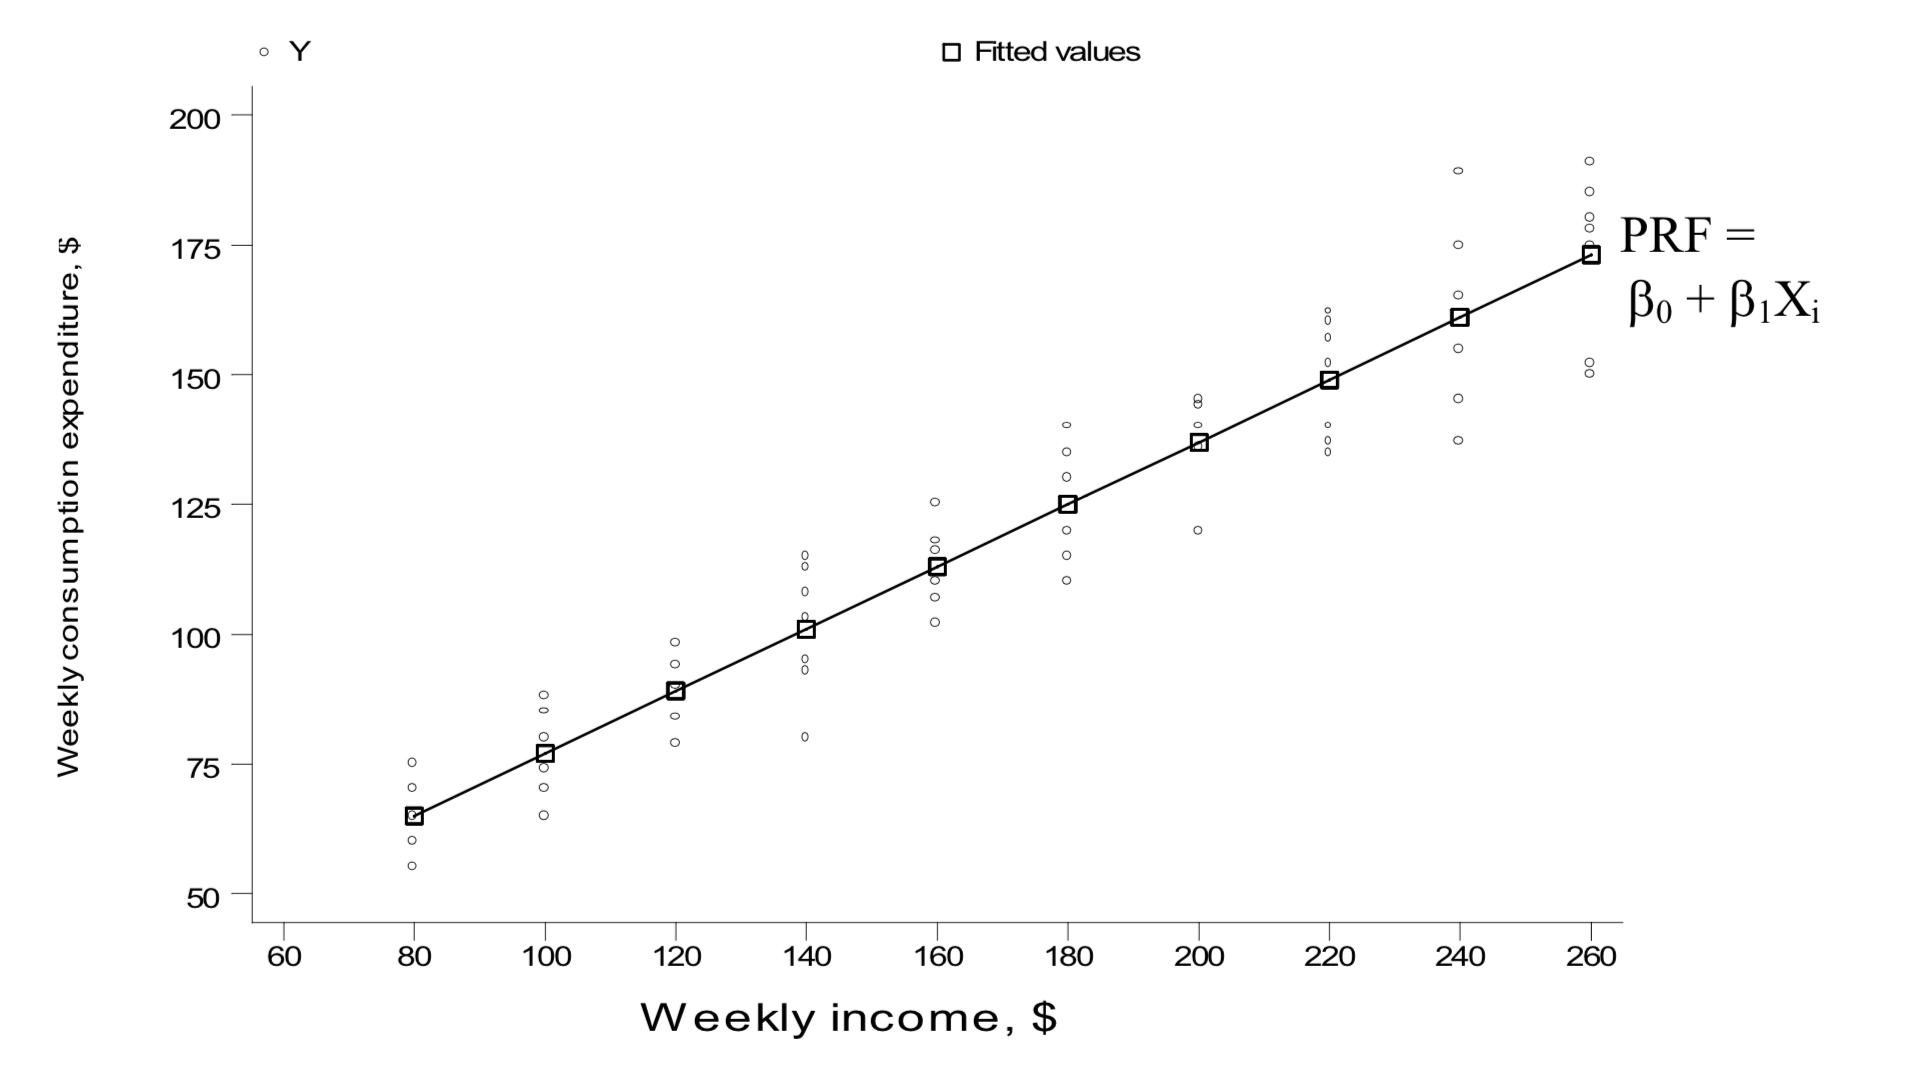
\includegraphics[scale=0.35] {images/prf_plot}}
\caption{Example Population Regression Function: $f(X_i)= \E(Y_i | X_i ) = \beta_0 + \beta_{1} X_i$}
\label{fig:prf}
\end{figure}

\subsection{Properties of the random error term $\boldsymbol \varepsilon_i$}
\textbf{Assumption A2}: \emph{Zero Conditional Mean Error}.  
\label{a:a2}
The conditional mean, or conditional expectation, of the random error terms $\varepsilon_i $ 
for any given value $X_i$ of the regressor $X$ is equal to zero. That is
\begin{flalign}
\E[\varepsilon \mid X] = 0 \text{ or } \E[\varepsilon_i \mid X_i] = 0 \; \forall i
\label{eqn:zcme}
\end{flalign}

\bigskip
\noindent
This assumption is saying two things: 
\begin{enumerate}
\item The conditional mean of the random error term $\varepsilon$ is the same for all population values of $X$;  it does not depend, either linearly or nonlinearly on $X$.
\item The common conditional population mean of $\varepsilon$ for all values of $X$ is zero.
\end{enumerate}

\bigskip
\noindent
There are several implications of assumption A2. The first implication is that the \emph{unconditional mean} of the population values of the random error term $\varepsilon$
equals zero. That is
\begin{flalign}
\E[\varepsilon \mid X] &= 0 \Rightarrow  \E[\varepsilon] = 0 \\
\E[\varepsilon_i \mid X_i] &= 0 \Rightarrow  \E[\varepsilon_i] = 0
\end{flalign}

\bigskip
\noindent
This follows from the \emph{law of iterated expectation}, which states that $\E[\E[\varepsilon \mid X]] =  \E[\varepsilon]$. In particular, since $\E[\varepsilon \mid X] = 0$ by A2, we see that 
\begin{flalign}
\E[\varepsilon] &= \E[\E[\varepsilon \mid X]]  \qquad \qquad \qquad \mathrel{\#} \text{law of iterated expectation} \\
&= \E[0]   \; \; \; \qquad  \qquad \qquad \qquad \mathrel{\#} \text{ since } \E[\varepsilon \mid X] = 0  \text{ (A2)} \\
&= 0  \qquad \qquad  \qquad \qquad \qquad \mathrel{\#} \text{ since } \E[c] = c \text{ for constant } c
\label{eqn:e=0}
\end{flalign} 

\bigskip
\noindent
One way to think about this is that if the conditional mean of $\varepsilon$ for each and every population value of $X$ equals zero, then the mean of these zero conditional means 
must also be zero.

\bigskip
\noindent
Another implication of A2 is that the population values $X_i$ of the regressor $X$ and $\varepsilon_i$ of the random error term $\varepsilon$ have zero covariance.
That is,  the population values of $X$ and $\varepsilon$ are uncorrelated. That is, 
\begin{flalign}
\E[\varepsilon \mid X] &= 0 \Rightarrow \Cov(X,\varepsilon) = \E[X\varepsilon] = 0  \\
\E[\varepsilon_i \mid X_i] &= 0 \Rightarrow \Cov(X_i,\varepsilon_i) = \E[X_i \varepsilon_i] = 0 
\end{flalign} 

\bigskip
\noindent
We can see this as follows:
\begin{flalign}
\Cov(X_i,\varepsilon_i) &= \E\big [ [X_i - \E[X_i]] [\varepsilon_i - \E[\varepsilon_i] ]\big ] \:\qquad \qquad \mathrel{\#} \text{definition of covariance} \\
&= \E{[X_i - \E[X_i]]\varepsilon_i}  \;\;\;\quad \quad \qquad \qquad \qquad \mathrel{\#} \text{since } \E[\varepsilon_i] = 0 \text{ by A2} \\
&= \E[X_i \varepsilon_i  - \E[X_i]\varepsilon_i]  \;\quad \quad \qquad \qquad \qquad \mathrel{\#} \text{multiply through} \\
&=  \E[X_i \varepsilon_i] -  \E[X_i ]\E[ \varepsilon_i]  \quad \qquad \qquad \qquad \mathrel{\#} \text{since } \E[X_i] \text{ is a constant} \\
&= \E[X_i  \varepsilon_i ]   \:\:\: \qquad \qquad \qquad \qquad \qquad \qquad \mathrel{\#} \text{since } \E[ \varepsilon_i]  = 0 \text{ by A2} \\
&= \E[X_i] E[ \varepsilon_i ]  \; \quad \qquad \qquad \qquad \qquad \qquad \mathrel{\#} \E[XY] = \E[X] \cdot \E[Y]  \\
&= 0                                    \:   \qquad \qquad  \qquad \qquad \quad \qquad \qquad \qquad \mathrel{\#} \text{since } \E[\varepsilon_i] = 0 \text{ by A2} 
\end{flalign} 

\bigskip
\noindent
A third implication of A2 is the conditional mean of the population $Y_i$ values corresponding to a given value $X_i$ of the regressor $X$ equals 
the population regression function (PRF)  $f(X_i) = \beta_0 + \beta_{1}X_i$. This itself has a key implication, namely, that 

\begin{flalign}
\E(\varepsilon \mid X)      &= 0 \Rightarrow  \E(Y \mid X) = f(X) = \beta_0 + \beta_{1}X \text{ and} \\
\E(\varepsilon_i \mid X_i) &= 0 \Rightarrow  \E(Y_i \mid X_i) = f(X_i) = \beta_0 + \beta_{1}X_i  \qquad   \forall i
\end{flalign}

\bigskip
\noindent
The proof of this is fairly simple. Recall that by assumption $Y_i = \beta_0 + \beta_{1}X_i + \varepsilon_i$ for $i = 1 \hdots N$. Then

\begin{flalign}
Y_i  &= \beta_0 + \beta_{1}X_i + \varepsilon_i    \;\;\:\:  \quad \qquad \qquad \qquad \mathrel{\#} \text{Linear assumption, A1} \\
\E[Y_i  | X_i] &= \E[\beta_{0} +  \beta_{1}X_i + \varepsilon_i  | X_i]                     \:  \qquad   \qquad \quad \mathrel{\#} \text{Expectation conditioned on } X_ i \\
 &= \E[\beta_{0} +  \beta_{1}X_i |  X_i ] + \E[\varepsilon_i  | X_i]       \;\:   \qquad \mathrel{\#}  \E[X + Y | Z] = \E[X | Z] + \E[Y | Z] \\
 &= \E[\beta_{0} + \beta_{1}X_i | X_i]  \: \quad \qquad  \qquad \qquad \mathrel{\#} E[\varepsilon_i |  X_i]  = 0  \text{ by A2}  \\
 &= \E[\beta_{0} | X_i] + \E[\beta_{1}X_i |  X_i]   \;\; \quad  \quad \qquad \mathrel{\#}  \E[X + Y | Z] = \E[X | Z] + \E[Y | Z] \\
 &= \beta_0 + \E[ \beta_{1}X_i |  X_i]         \:   \quad  \qquad \qquad \qquad \mathrel{\#}  \E[\beta_0 | X_i] = \beta_0 \text{ for constant } \beta_0 \\
 &= \beta_0 + \E[ \beta_{1} |  X_i] \E[X_i  | X_i]   \: \:  \qquad \qquad \mathrel{\#} \E[XY |  Z] = \E[X | Z] \cdot  \E[Y | Z]  \label{eqn:epectation} \\
 &= \beta_0 + \beta_{1}  \E[X_i |  X_i]                         \: \quad  \qquad \qquad \qquad \mathrel{\#}  \E[\beta_1 | X_i ] = \beta_1  \text{ for constant } \beta_1\\
 \E[Y_i |  X_i]  &= \beta_{0} + \beta_{1}X_i           \qquad \qquad \qquad  \qquad \qquad \mathrel{\#} \E[X_i |  X_i] = X_i  
\end{flalign}

\noindent
Note that in Equation \ref{eqn:epectation} $X$ and $Y$ ($\beta_1$ and $X_i$) are assumed to be independent.

\bigskip
\noindent
An amazing result really. But what we really want to do is estimate the population parameters $\beta_0$ and $\beta_1$. How do we do that? To get there we will need some more 
machinery. 

\newpage
\bibliographystyle{ieeetr}
\bibliography{/Users/dmm/papers/bib/ml}



\end{document} 
